%\documentclass[../../main.tex]{subfiles}
\documentclass[../../../informe/src/main.tex]{subfiles}

\begin{document}
\section{Ejercicio 3}

\subsection{Decoder}
El decoder es un circuito lógico que permite convertir información binaria (n bits), a $2^{n}$ salidas .
Se implementó un decoder de  de 2 entradas y cuatro salidas, de la siguiente manera:
\begin{figure}[H]
\centering
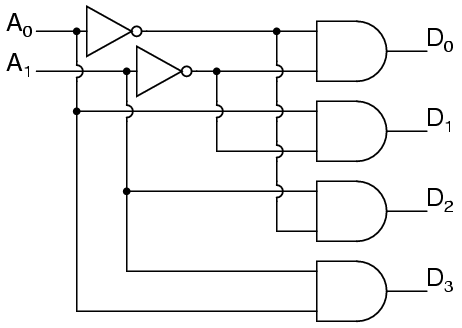
\includegraphics[width=0.4\textwidth]{imagenes/decoder.png}
\caption{Implementasión Decoder 4 salidas} \label{fig=decoder}
\end{figure}


Cuya tabla de verdad es:

\begin{table}[h]
\begin{center}
\begin{tabular}{|l|l|l|l|l|l|}
\hline
$A_{0}$ & $A_{1} $ & $D_{0}$  &  $D_{1}$ & $D_{2}$ & $A_{3}$\\
\hline \hline
0 & 0 & 1 & 0 & 0 & 0 \\ \hline
0 & 1 & 0 & 0 & 1 & 0 \\ \hline
1 & 0 & 0 & 1 & 0 & 0 \\ \hline
1 & 1 & 0 & 0 & 0 & 1 \\ \hline

\end{tabular}
\caption{Tabla de verdad del Decoder} 
\label{tab=decTab}
\end{center}
\end{table}

\subsection{Mux}

Los mux son circuitos lógicos que permiten poner a la salida una de las entradas.
Se pidió la implementación de un mux de 4 entradas, para ellos se realizó un mux de 2 entradas y a partir de él, se construyó el de cuatro salidas.

\begin{figure}[H]
\centering
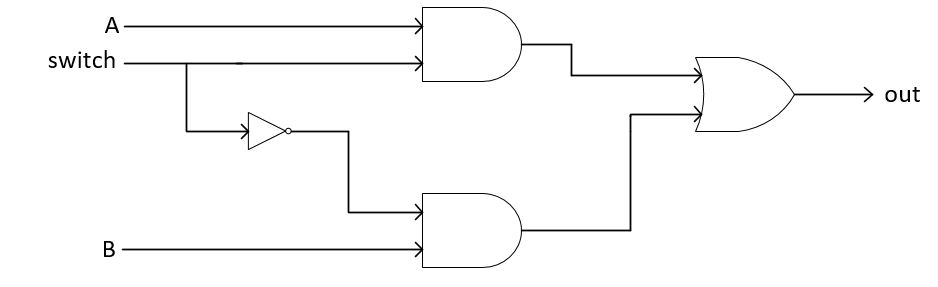
\includegraphics[width=0.8\textwidth]{imagenes/mux2.png}
\caption{Implementasión mux 2 entradas} \label{fig=mux2}
\end{figure}

\begin{table}[h]
\begin{center}
\begin{tabular}{|l|l|}
\hline
Switch & Out\\
\hline \hline
0 & B  \\ \hline
1 & A  \\ \hline


\end{tabular}
\caption{Tabla de verdad del Decoder} 
\label{tab=decTab}
\end{center}
\end{table}

\begin{figure}[H]
\centering
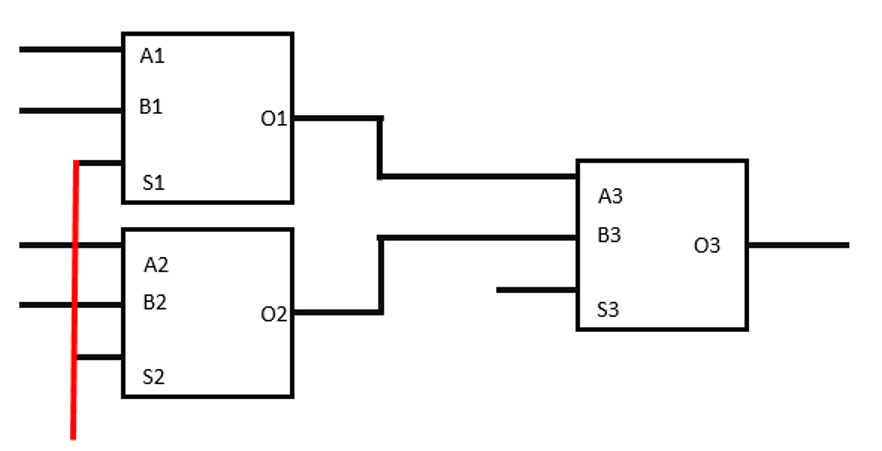
\includegraphics[width=0.8\textwidth]{imagenes/mux4.png}
\caption{Implementasión mux 4 entradas, las cajas son mux de dos entradas. Donde A y B son entrada y S es la selección} \label{fig=mux4}
\end{figure}

\begin{table}[h]
\begin{center}
\begin{tabular}{|l|l|l|}
\hline
$S_{1}$ y $S_{2}$ & $S_{3}$  & $O_{3}$\\
\hline \hline
0 & 0 & $B_{2}$  \\ \hline
0 & 1 & $B_{1}$  \\ \hline
1 & 0 & $A_{2}$  \\ \hline
1 & 1 & $A_{1}$  \\ \hline

\end{tabular}
\caption{Tabla de verdad del Mux de 4 entradas} 
\label{tab=mux4tab}
\end{center}
\end{table}





\section{Ejercicio 4}
\end{document}
